\documentclass[a4paper,AutoFakeBold,AutoFakeSlant]{ctexart}
\usepackage[a4paper,left=3cm,right=3cm,top=2.5cm,bottom=2.5cm]{geometry}
\usepackage{graphicx}
\usepackage{pythonhighlight}
\usepackage[mathscr]{eucal}
\usepackage{mathrsfs}
\usepackage{booktabs}
\usepackage{capt-of} 
\usepackage{hyperref} 
\usepackage{abstract}
\usepackage{amsmath}
\usepackage{listings}
\usepackage{color}
\usepackage{caption}
\usepackage{subfigure}
\usepackage{enumerate}
\usepackage{amsfonts} 
\usepackage{CJK,CJKnumb}
\usepackage{float}
% \usepackage{gbt7714}
\usepackage{framed}


\newcommand{\song}{\CJKfamily{song}}    % 宋体   (Windows自带simsun.ttf)
\newcommand{\fs}{\CJKfamily{fs}}        % 仿宋体 (Windows自带simfs.ttf)
\newcommand{\kai}{\CJKfamily{kai}}      % 楷体   (Windows自带simkai.ttf)
\newcommand{\hei}{\CJKfamily{hei}}      % 黑体   (Windows自带simhei.ttf)
\newcommand{\li}{\CJKfamily{li}}        % 隶书   (Windows自带simli.ttf) 
\newcommand{\ssong}{\CJKfamily{STSong}}

\xeCJKsetup{SlantFactor = 0.3}
% \xeCJKsetup{SlantFactor = -0.7}
\setCJKmainfont[BoldFont=simhei.ttf, SlantedFont=simkai.ttf]{simsun.ttc}



% -- 中文字体 --
%\setCJKmainfont{Microsoft YaHei}  % 微软雅黑
%\setCJKmainfont{YouYuan}  % 幼圆
%\setCJKmainfont{NSimSun}  % 新宋体
%\setCJKmainfont{KaiTi}    % 楷体
% \setCJKmainfont{SimSun}   % 宋体
%\setCJKmainfont{SimHei}   % 黑体
% \setCJKfamilyfont{hwsong}{STSong}
 
% -- 英文字体 --
% \setmainfont{Times New Roman}
% \setmainfont{DejaVu Sans}
% \setmainfont{Latin Modern Mono}
% \setmainfont{Consolas}
% \setmainfont{Courier New}


\usepackage{xcolor}  	%高亮使用的颜色
\definecolor{commentcolor}{RGB}{85,139,78}
\definecolor{stringcolor}{RGB}{206,145,108}
\definecolor{keywordcolor}{RGB}{34,34,250}
\definecolor{backcolor}{RGB}{220,220,220}

\usepackage{accsupp}	
\newcommand{\emptyaccsupp}[1]{\BeginAccSupp{ActualText={}}#1\EndAccSupp{}}

\usepackage{listings}
\lstset{						%高亮代码设置
	language=python, 					%Python语法高亮
	linewidth=0.95\linewidth,      		%列表list宽度
	%basicstyle=\ttfamily,				%tt无法显示空格
	commentstyle=\color{commentcolor},	%注释颜色
	keywordstyle=\color{keywordcolor},	%关键词颜色
	stringstyle=\color{stringcolor},	%字符串颜色
	%showspaces=true,					%显示空格
	numbers=left,						%行数显示在左侧
	numberstyle=\tiny\emptyaccsupp,		%行数数字格式
	numbersep=5pt,						%数字间隔
	frame=single,						%加框
	framerule=0.1pt,						%划线
	escapeinside=@@,					%逃逸标志
	emptylines=1,						%
	xleftmargin=3em,					%list左边距
	backgroundcolor=\color{backcolor},	%列表背景色
	tabsize=4,							%制表符长度为4个字符
	% gobble=4							%忽略每行代码前4个字符
}




\renewcommand{\abstractname}{}    % clear the title
\renewcommand{\absnamepos}{empty}
%去除摘要两边缩进
\makeatletter
  \renewenvironment{abstract}{%
      \if@twocolumn
        \section*{\abstractname}%
      \else
        \small
        \begin{center}%
          {\bfseries \abstractname\vspace{-.5em}\vspace{\z@}}%
        \end{center}%
      \fi}
      {}
  \makeatother
  \lstset{
    language=Matlab,
    keywords={break,case,catch,continue,else,elseif,end,for,function,
       global,if,otherwise,persistent,return,switch,try,while},
    basicstyle=\ttfamily,
    keywordstyle=\color{blue}\bfseries,
    commentstyle=\color{dkgreen},
    stringstyle=\color{dkpurple},
    backgroundcolor=\color{white},
    tabsize=4,
    showspaces=false,
    showstringspaces=false
 }

\title{\textbf{\textsf{{\textsf{HW4} \heiti{数学建模报告}}}}} 
\author{\ssong PB19151769~~~~~~马宇骁}
\date{}


\begin{document}



\maketitle


\begin{abstract}\zihao{-4} \kaishu
\noindent
\textbf{\heiti 摘要:} 利用国家统计局网站 http://www.stats.gov.cn/ 上的月度数据,
建立数学模型,分析“粮食、
经济作物、畜产品、水产品、蔬菜、水果”这六大类农产品集贸市场价格之间的联系,以
及他们对于居民消费价格指数 CPI 的影响.
\newline
\textbf{\heiti 关键词:} 农产品,居民消费价格指数,CPI
\end{abstract}

\section{背景}
从2020 年,全国工作重心转向两个主要的
方面:保障医疗物资、助力医疗救助;保障人民生活物
资、维护安定社会环境。生活物资的保障,是关系到每位
老百姓一日三餐、衣食住行的国计民生的大事。\cite{何叶20202020}

生活物资需求主要来源于一日三餐的食物,主要依靠
农产品提供保障。粮食,是老百姓生存最基本的能量和食物的来源,更
是一个国家经济发展的基础。而经济作物作为为轻工业提
供原料的作物,不但经济价值很高,也是人民重要的生活
保障物资。

除去粮食作物和经济作物,畜产品和水产品也在老百
姓餐桌上也扮演了非常重要的角色。畜产品主要包括肉类
(如猪、牛、羊、鸡、鸭、鹅、兔等)、蛋类(如鸡蛋、鸭
蛋、鹅蛋、鸽子蛋、鹌鹑蛋等)、奶类(如牛奶、羊奶、马
奶等)、蜂产品(如蜂蜜、蜂花粉、蜂王浆等)及其他副产
品。水产品主要包括淡水产品和海水产品两大类,按照生
物学特征可分为鱼类(如草鱼、鲤鱼等)、甲壳动物类(如
明虾、海蟹等)、软体动物类(如鲍鱼、扇贝等)、棘皮动
物类(如海胆、海参等)、腔肠动物类(如海蜇等)及其他
水产品。

粮食作物主要为生命提供葡萄糖以转换可利用的能
量,畜产品和水产品为人们提供生命活动必不可少的蛋白
质。蔬菜和水果作为人体食物主要的补充来源,主要补充
人体所需要的维生素、纤维素和矿物质。蔬菜和水果所含
的多种天然化学物质是富含生物活性的化合物,保护植物
免受自然界里面细菌、病毒和真菌的侵害。这些天然化学
物质的生活活性机理还不能被人们所完全认识。但其对人
体预防和对抗各种病原体入侵、吸收毒素、器官衰老和组
织癌变所起到的作用,已经为大家所认知和利用。


\section{分析}
从国家统计局的数据库中下载从2013年1月至今(2022年)的六大类农产品集贸市场价格月度数据\cite{数据}。由于每类数据中
所包含的农产品种类很多,因此,只取前三个价格当期数据作图并展示如下:
% \begin{figure}[htbp]
%   \centering
%   \begin{minipage}[t]{0.48\textwidth}
%   \centering
%   \includegraphics[width=6.5cm]{liang.png}
%   \caption{粮食集贸市场价格}
%   \label{f1}
%   \end{minipage}
%   \begin{minipage}[t]{0.48\textwidth}
%   \centering
%   \includegraphics[width=6.5cm]{jing.png}
%   \caption{经济作物集贸市场价格}
%   \label{f2}
%   \end{minipage}
% \end{figure}

\begin{figure}[H]
  \centering
  \includegraphics[scale=0.475]{liang.png}
  \caption{粮食集贸市场价格}
  \label{f1}
\end{figure}

看出粮食的价格基本在稳步上升,但在最近两年有波动。

\begin{figure}[H]
  \centering
  \includegraphics[scale=0.35]{jing.png}
  \caption{经济作物集贸市场价格}
  \label{f2}
\end{figure}

经济作物的价格在近十年价格变动不明显。

\begin{figure}[H]
  \centering
  \includegraphics[scale=0.35]{xu.png}
  \caption{畜产品集贸市场价格}
  \label{f3}
\end{figure}

畜产品价格具有周期性,详细分析见马宇骁的猪周期的分析\cite{数学建模HW2实验报告},该篇文章详细分析了
畜产品价格的周期性的原因原理和预测方式。

\begin{figure}[H]
  \centering
  \includegraphics[scale=0.35]{shui.png}
  \caption{水产品集贸市场价格}
  \label{f4}
\end{figure}

水产品的整体价格栽在提升,且趋势愈发明显。

\begin{figure}[H]
  \centering
  \includegraphics[scale=0.35]{shu.png}
  \caption{蔬菜集贸市场价格}
  \label{f5}
\end{figure}

从图\ref{f5}可以看出蔬菜中,大白菜的价格稍有提升,黄瓜和西红柿的价格有明显周期性。

\begin{figure}[H]
  \centering
  \includegraphics[scale=0.35]{guo.png}
  \caption{水果集贸市场价格}
  \label{f6}
\end{figure}

图\ref{f6}显示出水果的价格在近年的变动,也有周期趋势。

CPI数据是采用的以每一个上月为100计算的数据(由于数据库CPI的数据只有从2016年1月份
开始的,因此只展示2016.1之后的数据,第二个建模也是如此),原始数据绘图如下:
\begin{figure}[htbp]
  \centering
  \includegraphics[scale=0.7]{cpi.pdf}
  \caption{CPI}
  \label{f7}
\end{figure}

假设以2015.12为CPI为100,做累计CPI转化,这样得到的调整CPI数据进行绘制如图\ref{f8}.
\begin{figure}[htbp]
  \centering
  \includegraphics[scale=0.7]{cpi_adj.pdf}
  \caption{调整CPI}
  \label{f8}
\end{figure}

至此,数据初分析步骤结束,引入两个建模模型。


\section{建模}

由于要分析的6个类里面的项目过多,在建模时考虑简化将每个类中抽出一组出来作为特征数据进行建模: 
小麦,花生仁,活猪,鲤鱼,黄瓜,香蕉。


\subsection{农产品集贸市场价格之间的联系}
使用向量自回归(vector autoregressive, VAR)模型。\cite{tsay2005analysis}

VAR模型是用模型中所有当期变量对所有变量的若干滞后变量进行回归。
即
向量自回归模型把系统中每一个内生变量作为系统中所有内生变量的滞后值的函数来构造模型,从而实现了将单变量自回归模型推广到由多元时间序列变量组成的“向量”自回归模型。

VAR模型常用于预测相互联系的时间序列系统以及分析随机扰动对变量系统的动态影响,主要应用于宏观经济学。是处理多个相关经济指标的分析与预测中最容易操作的模型之一。

由于向量自回归模型把每个内生变量作为系统中所有内生变量滞后值的函数来构造模型,从而避开了结构建模方法中需要对系统每个内生变量关于所有内生变量滞后值的建模问题。

\subsubsection{VAR模型}
模型的基本形式是弱平稳过程的自回归表达式,描述的是在同一样本期间内的若干变量可以作为它们过去值的线性函数。

\begin{equation}
  Y_{t}=\Phi_{0}+\Phi_{1} Y_{t-1}+\cdots+\Phi_{p} Y_{t-p}+B X_{t}+\varepsilon_{t}, \quad t=1,2, \cdots, T
\end{equation}
其中,
\begin{equation*}
  \begin{array}{c}
    Y_{t}=\left(\begin{array}{c}
    y_{1 t} \\
    y_{2 t} \\
    \vdots \\
    y_{k t}
    \end{array}\right), \varepsilon_{t}=\left(\begin{array}{c}
    \varepsilon_{1 t} \\
    \varepsilon_{2 t} \\
    \vdots \\
    \varepsilon_{k t}
    \end{array}\right), \quad \Phi_{0}=\left(\begin{array}{c}
    \phi_{10} \\
    \phi_{20} \\
    \vdots \\
    \phi_{k 0}
    \end{array}\right) \\

    \Phi_{i}=\left(\begin{array}{cccc}
    \phi_{11}(i) & \phi_{12}(i) & \cdots & \phi_{1 k}(i) \\
    \phi_{21}(i) & \phi_{22}(i) & \cdots & \phi_{2 k}(i) \\
    \vdots & \vdots & \ddots & \vdots \\
    \phi_{k 1}(i) & \phi_{k 2}(i) & \cdots & \phi_{k k}(i)
    \end{array}\right), \quad i=1,2, \cdots, p
    \end{array}
\end{equation*}

\begin{itemize}
  \item $Y_t$表示 k 维内生变量列向量
  \item $Y_{t-i}$​,i=1,2,⋯,p 为滞后的内生变量
  \item $X_t​$ 表示 d 维外生变量列向量,它可以是常数变量、线性趋势项或者其他非随机变量
  \item p 是滞后阶数
  \item T 为样本数目
  \item $\Phi_i$即 $\Phi _1,\Phi _2\cdots ,\Phi _p$ 为  k $\times$ k  维的待估矩阵
  \item B 为 k $\times$ d 维的待估矩阵
  \item $\varepsilon_t​ \sim N(0,\Sigma)$ 为 k 维白噪声向量,它们相互之间可以同期相关,但不与自己的滞后项相关($\varepsilon _t$ 独立同分布,而 $\varepsilon _t$ ​ 中的分量不要求相互独立),也不与上式中右边的变量相关。 $\Sigma$  是 $\varepsilon _t$ ​ 的协方差矩阵, 是一个  k $\times$ k  的正定矩阵。
\end{itemize}

VAR模型的特点:
\begin{enumerate}
  \item 不以严格的经济理论为依据。在建模过程中只需明确两件事:①共有哪些变量是相互有关系的,把有关系的变量包括在VAR模型中;②确定滞后期 p。使模型能反映出变量间相互影响的绝大部分。
  \item VAR模型对参数不施加零约束。(对无显着性的参数估计值并不从模型中剔除,不分析回归参数的经济意义。)
  \item VAR模型的解释变量中不包括任何当期变量,所有与联立方程模型有关的问题在VAR模型中都不存在(主要是参数估计量的非一致性问题)。
  \item VAR模型的另一个特点是有相当多的参数需要估计。比如一个VAR模型含有三个变量,最大滞后期 p=3,则有27个参数需要估计。当样本容量较小时,多数参数的估计量误差较大。
  \item 无约束VAR模型的应用之一是预测。由于在VAR模型中每个方程的右侧都不含有当期变量,这种模型用于样本外一期预测的优点是不必对解释变量在预测期内的取值做任何预测。
  \item 用VAR模型做样本外近期预测非常准确。做样本外长期预测时,则只能预测出变动的趋势,而对短期波动预测不理想。
\end{enumerate}

\subsubsection{数据建模}
先计算数据之间的相关系数,结果如下:
\begin{figure}[htbp]
  \centering
  \includegraphics[scale=0.875]{corr.pdf}
  \label{f9}
\end{figure}

存在一定程度的线性相关。
接下来对6个因子的原始数据进行平稳性检验,也就是ADF检验。
VAR模型要求所有因子数据同阶协整,也就是6个因子里面如果有一个因子数据不平稳,就要全体做差分,一直到平稳为止。

利用statsmodels.api中的tsa.stattools.adfuller进行检验,结果小麦的p-Value为\\0.9988888206197162远大于0.05即不平稳,因此先对全体做
一阶差分。此时,6个因子的p-Value为:
\begin{quote}
  4.4230116313574625e-12,\\
  2.501592689892194e-07,\\
  1.7504784916922888e-11,\\
  2.081139096614198e-07,\\
  1.0106031873420553e-14,\\
  1.3650732557033655e-11
\end{quote}
这时全部通过ADF检验,即一阶差分数据平稳。

继续做协整检验
python里面的协整检验通过coint()这个函数进行的,返回p-Value值,越小,说明协整关系越强。
对6个因子差分后数据两两进行协整检验,返回p-Value如下:
\begin{quote}
  3.794476144670872e-11,\\
 5.6650734297401955e-11,\\
 4.197438490154251e-11,\\
 1.571125632531838e-10,\\
 2.3952266770030205e-11,\\
 1.4050118223059445e-06,\\
 3.323609186664604e-06,\\
 2.4405406556407465e-06,\\
 1.6947364044637295e-06,\\
 2.134621409174666e-11,\\
 9.49864513220687e-11,\\
 2.0062078357777857e-10,\\
 1.626602232542773e-06,\\
 2.4495993845569412e-06,\\
 8.080175996078994e-13
\end{quote}
发现这所有关系均存在长期均衡关系,VAR 模型应采用一阶差分后的数据构建。

使用2013年1月至2021年12月的数据进行VAR模型构建,将2022年数据留作预测检验。

先确定滞后项阶数:

通过statsmodels.tsa.vector\_ar.var\_model.VAR中的select\_order()函数实现,综合考虑,采用 1 阶滞后系数作为模型参数。(输出结果如下表,*代表最优参数)
\begin{figure}[htbp]
  \centering
  \includegraphics[scale=0.875]{lag.pdf}
  \label{f10}
\end{figure}

经过拟合VAR(1),输出结果为:
\begin{figure}[H]
  \centering
  \includegraphics[scale=0.63]{var1.pdf}
  \label{f11}
\end{figure}

即,写成矩阵形式,模型最终为:
\begin{small}
\begin{equation*}
  \begin{aligned}
    \left(\begin{array}{c}
      y_{1 t} \\
      y_{2 t} \\
      y_{3 t} \\
      y_{4 t} \\
      y_{5 t} \\
      y_{6 t}
    \end{array}\right)&=\left(\begin{array}{c}
      e_{1} \\
      e_{2} \\
      e_{3} \\
      e_{4} \\
      e_{5} \\
      e_{6}
    \end{array}\right)+\left(\begin{array}{c}
      0.003006 \\
      0.000407 \\
      0.127205 \\
      0.011866 \\
      0.038110 \\
      0.002724
    \end{array}\right)\\&+\left(\begin{array}{cccccc}
      0.163221 & -0.029237 & 0.001539 & 0.000521 & 0.007118 & -0.011380\\
      0.204820 & 0.505980  & 0.016170 &-0.036150 & -0.034109 & -0.093127\\
      -20.065400 &0.142134 & 0.270497& -1.066723& 0.136125& -0.715172\\
      0.987921 &0.126892  &0.003195  &0.525357 &-0.074237  &-0.091176 \\
      -4.706545 &-0.742301 &0.022692 & -0.329610 &0.318474 & -0.818694\\
      2.281493 & 0.134317& 0.000739& -0.108945&0.017197  &0.334841
    \end{array}\right)
    \left(\begin{array}{c}
      y_{1, t-1} \\
      y_{2, t-1} \\
      y_{3, t-1} \\
      y_{4, t-1} \\
      y_{5, t-1} \\
      y_{6, t-1}
    \end{array}\right)
  \end{aligned}
\end{equation*}
\end{small}
其中, $y_1, y_2, y_3, y_4, y_5, y_6$ 为六大类农产品集贸市场价格(小麦,花生仁,活猪,鲤鱼,黄瓜,香蕉)的一阶差分。

接下来检验模型:

首先,先通过绘制残差项自相关图来观察自相关性。可以看到,6个变量基本都在边界范围内,无明显自相关性。
\begin{figure}[htbp]
  \centering
  \includegraphics[scale=0.53]{acf.pdf}
  \caption{acf}
  \label{f12}
\end{figure}

残差项自相关性检验通过Q检验(Ljung-Box 方法)实现,Q 检验的原假设为$H_0$:检验最大滞后项 m 的自相关系数为0,即$\hat{\rho_1} =\hat{\rho_2} = …… =\hat{\rho_m}=0$。在原假设成立的条件下,Q(m)服从自由度为m的卡方分布。
通过 statsmodels.tsa.stattools中的 acf()函数实现 Q 检验, p-Value返回如下:
\begin{quote}
[array([0.52740219, 0.4384854 , 0.49037819, 0.64767928, 0.77306447,
        0.79696484, 0.87616611, 0.87238704, 0.45788608, 0.55245569]),\\
 array([0.49107943, 0.74735034, 0.51245593, 0.61830119, 0.16763974,
        0.18792779, 0.23932733, 0.31682872, 0.36286832, 0.44770081]),\\
 array([0.47051762, 0.76221575, 0.52713904, 0.63919973, 0.73425818,
        0.80729527, 0.75780236, 0.81106089, 0.8668216 , 0.61634637]),\\
 array([0.25724948, 0.42584887, 0.5648922 , 0.26907737, 0.14589302,
        0.10697081, 0.15511247, 0.20354774, 0.22310506, 0.28581413]),\\
 array([0.79108719, 0.54843777, 0.5303361 , 0.35351412, 0.48682279,
        0.33834312, 0.43503051, 0.18594445, 0.2542709 , 0.30858343]),\\
 array([0.23637255, 0.02322106, 0.02940898, 0.06009484, 0.08360409,
        0.12794423, 0.18925959, 0.22232667, 0.1699084 , 0.0566266 ])]
\end{quote}
都大于0.05,证明无法拒绝原假设,可以证明变量的残差为白噪声。模型拟合十分良好。

利用statsmodels.tsa.vector\_ar.var\_model.VARResults的forecast做4步预测:
\begin{figure}[htbp]
  \centering
  \includegraphics[scale=0.475]{figfore.pdf}
  \caption{四步预测}
  \label{f13}
\end{figure}

将预测结果的差分值与最后一期
相加每一步在进行转换(转换代码见代码附录),将预测与拟合结果和原始的真实值一并作图展示如下:
\begin{figure}[htbp]
  \centering
  \includegraphics[scale=0.75]{predict.pdf}
  \caption{'Forecast vs Actuals'}
  \label{f14}
\end{figure}

基本重合,模型拟合良好。

\subsubsection{模型分析}
通过一阶差分的VAR(1)模型,从模型结果来看:

首先,每个农产品的集贸市场价格都与自身的上个月的价格十分相关,即,上个月的价格很可能影响到下个月的价格。

其次,通过一阶差分使得每个序列平稳后,呈现出来的结果表明:
\begin{itemize}
  \item 小麦价格的一阶差分与上个月的小麦、活猪、鲤鱼、黄瓜的一阶差分成正向的线性关系,与上个月的花生仁、香蕉的价格一阶差分有负向的线性关系;
  \item 花生仁价格的一阶差分与上个月的小麦、花生仁、活猪的一阶差分成正向的线性关系,与上个月的香蕉、鲤鱼、黄瓜的价格一阶差分有负向的线性关系;
  \item 活猪价格的一阶差分与上个月的花生仁、活猪、黄瓜的一阶差分成正向的线性关系,与上个月的小麦、鲤鱼、香蕉的价格一阶差分有负向的线性关系;
  \item 鲤鱼价格的一阶差分与上个月的小麦、花生仁、活猪、鲤鱼的一阶差分成正向的线性关系,与上个月的香蕉、黄瓜的价格一阶差分有负向的线性关系;
  \item 黄瓜价格的一阶差分与上个月的活猪、黄瓜的一阶差分成正向的线性关系,与上个月的小麦、花生仁、鲤鱼、香蕉的价格一阶差分有负向的线性关系;
  \item 香蕉价格的一阶差分与上个月的小麦、活猪、花生仁、香蕉、黄瓜的一阶差分成正向的线性关系,与上个月的鲤鱼的价格一阶差分有负向的线性关系;
  \item 所有自己的一阶差分都与自己的上个月一阶差分成正向线性关系。
\end{itemize}

这在经济学上可能是由于这些商品之间的互补品和替代品的关系在市场选择中呈现出来的规律。

\subsection{对于居民消费价格指数 CPI 的影响}
使用多元线性回归模型(multivariable linear regression model )。

多元线性回归模型通常用来研究一个应变量依赖多个自变量的变化关系,如果二者的以来关系可以用线性形式来刻画,则可以建立多元线性模型来进行分析。
多元线性回归模型通常用来描述变量y和x之间的随机线性关系,即:
\begin{equation}
y_i=\beta_{0}+\beta_{1} x_{1}+\ldots+\beta_{k} x_{k}+\xi_i
\end{equation}
式中,  $x_{1}, \cdots, x_{k}$  是非随机的变量;$y$ 是随机的因变量;  $\beta_{0}, \cdots, \beta_{k}$  是回归系数;  $\xi$  是随机误差项。

用矩阵表示为:
\begin{equation}
  y=\left(\begin{array}{l}
    y_{1} \\
    y_{2} \\
    \vdots \\
    y_{n}
    \end{array}\right) \quad x=\left(\begin{array}{cccc}
    1 & x_{11} & \ldots & x_{k 1} \\
    1 & x_{12} & \ldots & x_{k 2} \\
    \vdots & \vdots & & \vdots \\
    1 & x_{1 n} & \ldots & x_{k n}
    \end{array}\right) \quad, \quad \beta=\left(\begin{array}{l}
    \beta_{0} \\
    \beta_{1} \\
    \vdots \\
    \beta_{k}
    \end{array}\right) \quad, \quad \xi=\left(\begin{array}{l}
    \varepsilon_{1} \\
    \varepsilon_{2} \\
    \vdots \\
    \varepsilon_{n}
    \end{array}\right)
\end{equation}

此时模型可以写作:
\begin{equation}
  y_i=X_i \beta+\xi_i
\end{equation}

建模步骤:
\begin{enumerate}
  \item 根据数据建立回归模型;
  \item 对模型进行显著性检验;
  \item 对模型进行回归诊断
\end{enumerate}

\subsubsection{数据建模}
由所选的特征列,加入常数1列,对2022年以前的CPI的调整值进行回归,结果如下方展示。
\begin{figure}[htbp]
  \centering
  \includegraphics[scale=0.725]{ols.pdf}
  \label{f15}
\end{figure}
回归方程为:
\begin{equation*}
  \hat{y_i} = 51.1172 + 16.8529x_{1i} -0.9055x_{2i} + 0.2714x_{3i} + 0.1127x{4i} + 0.1127x_{5i} + 1.2372x_{6i}
\end{equation*}

且模型的每个参数的p-Value都很小,参数显著,初步说明模型拟合不错。

对残差进行正态性检验:
\begin{figure}[htbp]
  % \centering
  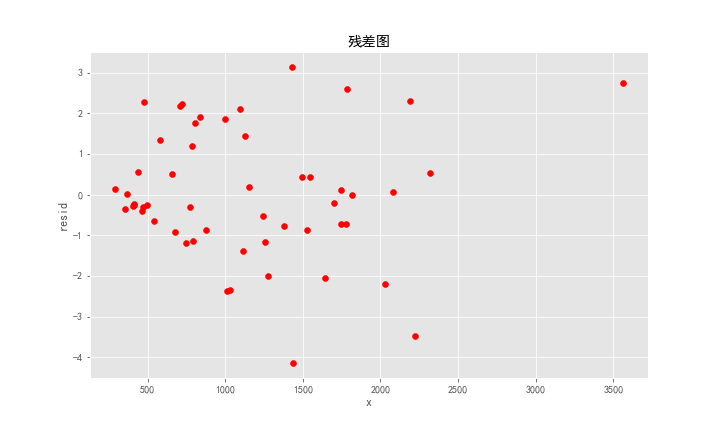
\includegraphics[scale=0.35]{res.pdf}
  \caption{残差质量分布}
  \label{f16}
\end{figure}

图\ref{f16}显示,残差的质量分布大致与零均值的正态分布相似,下面用QQ图\footnote{QQ plot的全称是Quantile-Quantile Plot,即分位数-分位数图。如果两个分布相似,则该Q-Q图趋近于落在y=x线上。如果两分布线性相关,则点在Q-Q图上趋近于落在一条直线上,但不一定在y=x线上。Q-Q图可以用来可在分布的位置-尺度范畴上可视化的评估参数。}再检验。
\begin{figure}[htbp]
  \centering
  \includegraphics[scale=0.35]{qq.pdf}
  \caption{残差QQ图}
  \label{f17}
\end{figure}

基本在一条直线上,可以认为残差符合零均值的正态分布。

以上步骤证明模型拟合很好,模型通过了所有检验,因此考虑将模型与真实之间做比较来证明农产品集贸市场价格对于居民消费价格指数 CPI 的影响模型
的准确性。
\newpage

\subsubsection{模型分析}
此时,对于模型做4步预测结果如下:
\begin{quote}
  113.203838\\
  112.681031\\
  114.567686\\
  115.334756
\end{quote}

真实情况为:
\begin{quote}
  112.6169365064331,\\
 113.2926381254717,\\
 113.2926381254717,\\
 113.74580867797359
\end{quote}

\begin{figure}[htbp]
  \centering
  \includegraphics[scale=0.5]{predict2.pdf}
  \caption{'Forecast vs Actuals'}
  \label{f18}
\end{figure}

考虑到置信区间看到,基本上与原始数据契合。

最终,可以从模型中分析得到,CPI调整值与六大类农产品集贸市场价格存在关系,且除了经济作物花生价格是负相关,与其他
产品之间都存在正向的线性关系。

\section{结论}
通过两个模型对“粮食、
经济作物、畜产品、水产品、蔬菜、水果”这六大类农产品集贸市场价格之间的联系,以
及他们对于居民消费价格指数 CPI 的影响的结果可以看出,两个模型的拟合都非常好,都能够准确的
对于现在的情况做出预测,从而为相关从业者的分析和操作提供非常有效的工具来参考。

如果想要对未来再分析,需要更多的近期数据进行迭代,使得两个模型再次发挥作用。

随着农业信息化的发展,价格数据的采集逐渐实现了短剑个采集,因此今后的研究中可利用更加海量的数据进行
模拟预测,例如可利用每日价格数据进行预测,从而获得更加精确到超短期预测结果,或者利用周期更长的月度
价格进行预测,研究长期变化规律。\cite{屠星月2014基于时间序列与}

\section*{代码附录}
部分Python代码展示如下:
\begin{python}
import pandas as pd
import numpy as np
import matplotlib as mpl
import matplotlib.pyplot as plt
import statsmodels.api as sm
from scipy import stats
from scipy.stats import kstest
from statsmodels.graphics.tsaplots import plot_acf, plot_pacf
data = pd.read_excel('月度数据 .xls')
name = data.columns
data = data.reindex(index=data.index[::-1])
data.index = [i for i in range(len(data))]
cpid = (data[[name[0],name[1]]].copy(deep=True)).dropna()
cpid.index = [i for i in range(len(cpid))]

from datetime import datetime
cpid[name[0]] = pd.to_datetime(cpid[name[0]])

date = cpid[name[0]]
cpi = cpid[name[1]]
plt.plot(date,cpi)
plt.savefig('cpi.pdf')
plt.show()

cpi_adj = []
cpi_adj.append(cpi[0])
for i in range(len(cpi)-1):
    c = cpi_adj[i]*cpi[i+1]/100
    cpi_adj.append(c)
plt.plot(date,cpi_adj)
plt.savefig('cpi_adj.pdf')
plt.show() 

m1 = data[[name[3],name[6],name[8],name[12],name[15],name[18]]].copy(deep=True)
name1 = m1.columns

plt.rc('figure', figsize=(12, 7))
plt.text(0.01, 0.05, str(m1.corr().values), {'fontsize': 10}, fontproperties = 'monospace') # approach improved by OP -> monospace!
plt.axis('off')
plt.tight_layout()
# plt.savefig('corr.pdf')

adfResult1 = sm.tsa.stattools.adfuller(m1[name1[0]])
adfResult2 = sm.tsa.stattools.adfuller(m1[name1[1]])
adfResult3 = sm.tsa.stattools.adfuller(m1[name1[2]])
adfResult4 = sm.tsa.stattools.adfuller(m1[name1[3]])
adfResult5 = sm.tsa.stattools.adfuller(m1[name1[4]])
adfResult6 = sm.tsa.stattools.adfuller(m1[name1[5]])

m11 = m1.diff().dropna()
adfResult1 = sm.tsa.stattools.adfuller(m11[name1[0]])
adfResult2 = sm.tsa.stattools.adfuller(m11[name1[1]])
adfResult3 = sm.tsa.stattools.adfuller(m11[name1[2]])
adfResult4 = sm.tsa.stattools.adfuller(m11[name1[3]])
adfResult5 = sm.tsa.stattools.adfuller(m11[name1[4]])
adfResult6 = sm.tsa.stattools.adfuller(m11[name1[5]])

from statsmodels.tsa.stattools import coint
c=[]
for i in range(5):
    for j in range(i+1,6):
        c.append(coint(m11[name1[i]],m11[name1[j]])[1])

m10 = m11.head(len(m11)-5)
from statsmodels.tsa.vector_ar.var_model import VAR
mod = VAR(m10)
lag_order = mod.select_order()
print(lag_order.summary())
plt.rc('figure', figsize=(12, 7))
plt.text(0.01, 0.05, str(lag_order.summary()), {'fontsize': 10}, fontproperties = 'monospace') # approach improved by OP -> monospace!
plt.axis('off')
plt.tight_layout()
# plt.savefig('lag.pdf')

res = mod.fit(1)
res.summary()
# # 设置中文编码和符号的正常显示
# plt.rcParams["font.sans-serif"] = "SimHei"
# plt.rcParams["axes.unicode_minus"] = False
plt.rc('figure', figsize=(12, 20))
plt.text(0.01, 0.05, str(res.summary()), {'fontsize': 10}, fontproperties = 'monospace') # approach improved by OP -> monospace!
plt.axis('off')
plt.tight_layout()
# plt.savefig('var1.pdf')

# 绘制残差项自相关图,最大滞后系数=10
res.plot_acorr(nlags=10, resid=True, linewidth=6)
# plt.savefig('acf.pdf')
plt.show()

from statsmodels.tsa.stattools import acf
# 以USDCNY变量为例,调用acf函数获得Q检验结果
pvalue = [i for i in range(6)]
for i in range(6):
    (resid_acf, qstat, pvalue[i]) = acf(res.resid[i+1], nlags=10, qstat=True)

res.plot_forecast(4)
plt.savefig('figfore.pdf')
plt.show()

pred1 = res.forecast(m10.values,4)
pred =  []
p = [m1[name1[j]][len(m1)-5] for j in range(6)]
for i in range(4):
    pp = []
    for j in range(6):
        pp.append(p[j]+pred1[i][j])
    pred.append(pp)

m01 = m1.head(len(m1)-4)
for i in range(4):
    m01.loc[i+len(m01)] = pred[i]

    # import matplotlib as mpl
plt.style.use('default')
date1 = pd.to_datetime(data[name[0]])
# Plot
# plt.figure(figsize=(12,5), dpi=100)
for i in range(6):
    plt.plot(date1,m1.loc[:,name1[i]], label='oringin'+str(i+1))
    # plt.plot(test, label='actual')
    plt.plot(date1,m01.loc[:,name1[i]], label='forecast'+str(i+1))
# plt.fill_between(lower_series.index, lower_series, upper_series, 
#                  color='k', alpha=.15)
# plt.title('Forecast vs Actuals')
plt.legend(loc='upper left', fontsize=8)
# plt.savefig('predict.pdf')
plt.show()

m2 = data[[name[3],name[6],name[8],name[12],name[15],name[18]]].copy(deep=True)
m2 = m2.dropna().tail(len(cpi_adj))
m2['cpi_adj'] = cpi_adj
m2.index = [str(i) for i in range(len(m2))]
name2 = m2.columns
# m2.columns = [i for i in range(7)]
# m2.rename(columns={'6':'cpi_adj'})
y = m2[name2[6]].head(len(y)-4)
x = m2[[name2[i] for i in range(6)]].head(len(x)-4)
x.columns = [i for i in range(1,7)]
# from statsmodels.formula.api import ols
import statsmodels.api as sm
import statsmodels.formula.api as smf
# 小写的 ols 函数才会自带截距项,OLS 则不会
# 固定格式:因变量 ~ 自变量(+ 号连接)

x = sm.add_constant(x)
regression = sm.OLS(y, x) #用最小二乘法建模
model = regression.fit() #数据拟合
model.summary()
plt.rc('figure', figsize=(8, 5))
# plt.style.use('default')
plt.text(0.01, 0.05, str(model.summary()), {'fontsize': 10}, fontproperties = 'monospace') # approach improved by OP -> monospace!
plt.axis('off')
plt.tight_layout()
# plt.savefig('ols.pdf')

plt.rcParams.update({'figure.figsize':(15,6), 'figure.dpi':200})
residuals = pd.DataFrame(model.resid)
fig, ax = plt.subplots(1,2)
residuals.plot(title="Residuals", ax=ax[0])
residuals.plot(kind='kde', title='Density', ax=ax[1])
plt.savefig('res.pdf')
plt.show()

resid = model.resid
# plt.rcParams.update({'figure.figsize':(12,7), 'figure.dpi':100})
from statsmodels.graphics.api import qqplot

qqplot(resid, line='q', fit=True)
plt.savefig('qq.pdf')
plt.show()

test = m2
xtest = test[[name2[i] for i in range(6)]]
xtest = sm.add_constant(xtest)
pred = model.predict(exog=xtest)

import matplotlib.pyplot as plt
m22 = data[[name[0],name[1]]].dropna()
date2 = pd.to_datetime(m22[name[0]])

plt.plot(date2,cpi_adj, label='oringin')

plt.plot(date2,pred, label='forecast')

plt.legend(loc='upper left', fontsize=8)
plt.savefig('predict2.pdf')
plt.show()
\end{python}

% \bibliographystyle{gbt7714-numerical}
% % \bibliographystyle{7714-author-year}
\bibliographystyle{ieeetr}
\bibliography{bibl}

\end{document}